\subsection[Gestire classi multiple: OvR e OvO]{Gestire classi multiple: OvR e OvO}

%\subsubsection[Training e test set]{Training e test set}


\begin{frame}
	
	\frametitle{Gestire classi multiple}
	I problemi di classificazione non sono sempre riconducibili a due classi.\\
	La maggior parte degli algoritmi che prevedono delle probabilità o un punteggio per le classi è in grado di gestire automaticamente i problemi di classi multiple utilizzando due diverse strategie:
	
	\begin{itemize}
		\item \textbf{One Versus Rest (OvR)}: l'algoritmo confronta ogni classe con quelle rimanenti, creando un modello per ogni classe. La classe con la probabilità più elevata è quella che viene scelta; pertanto, se un problema deve trovare tre classi, anche l'algoritmo utilizza tre modelli.
		\item \textbf{One Versus One (OvO)}: in questo caso l'algoritmo compara a due a due le classi, creando un numero di modelli equivalente a $ \frac{n * (n-1)}{2}$, laddove $n$ è il numero delle classi (es: $n=5 \Rightarrow$ num modelli $=10$). La classe che viene scelta per la predizione, è quella che vince per numero di previsioni a suo vantaggio rispetto a tutte le altre (con un'analogia si può dire che è un po' come una classifica a punti fra squadre in un torneo).
	\end{itemize}
	
\end{frame}


\begin{frame}
	
	\frametitle{Gestire classi multiple: OvR e OvO a confronto}
	
	\begin{figure}[!htbp]
		\centering
		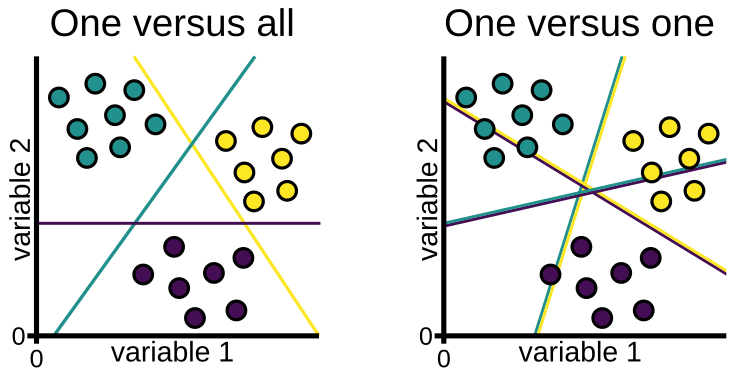
\includegraphics[width=0.85\linewidth]{images/supervised/multiple_classes/OvR_OvO.png}
		%\caption{}
	\end{figure}
	
	Ad esempio nel caso della \underline{\href{https://scikit-learn.org/stable/modules/generated/sklearn.linear_model.LogisticRegression.html}{regressione logistica}} in \underline{\href{https://scikit-learn.org/stable/modules/multiclass.html}{Scikit-learn}}, la strategia multiclasse proposta di default è quella One Versus All (One Versus Rest).
	
\end{frame}